\documentclass[tikz,border=7pt]{standalone}
\usepackage{amsmath}
\usetikzlibrary{positioning}
\tikzset{box/.style={draw,rectangle,rounded corners=2pt,minimum width=80mm,minimum height=50mm,align=left},port/.style={draw,circle,minimum size=5mm,inner sep=0pt}}
\begin{document}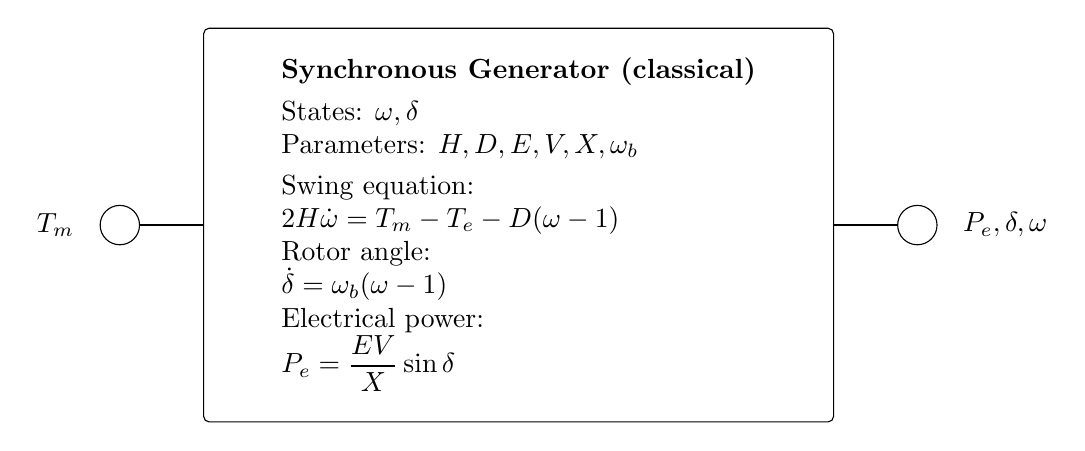
\begin{tikzpicture}
\node[box] (c) {\textbf{Synchronous Generator (classical)}\\[1mm]
States: $\omega,\delta$\\
Parameters: $H,D,E,V,X,\omega_b$\\[1mm]
Swing equation:\\
$\displaystyle 2H\dot\omega = T_m-T_e-D(\omega-1)$\\
Rotor angle:\\
$\displaystyle \dot\delta = \omega_b(\omega-1)$\\
Electrical power:\\
$\displaystyle P_e=\frac{EV}{X}\sin\delta$};
\node[port,left=8mm of c] (m) {};\node[port,right=8mm of c] (e) {};
\node[left=2mm of m] {$T_m$};\node[right=2mm of e] {$P_e,\delta,\omega$};
\draw[thick] (m)--(c.west);\draw[thick] (c.east)--(e);
\end{tikzpicture}\end{document}
